% Por hacer:
% Hacer la(s) gráficas en tikz

Como comentario adicional, si tenemos dos funciones integrables $f, g$, gracias a lo demostrado anteriormente, si expresamos el produto $f(x)g(x)$ de la siguiente manera:

\[
f(x)g(x) = \frac{1}{4}(f(x) + g(x))^2 - \frac{1}{4}(f(x) - g(x))^2
\]

\noindent entonces podremos demostrar que $f \cdot g$ es integrable. Sin embargo, ahora nos centraremos en estudiar otras propiedades. La demostración de $fg \in \Rint$ se deja como ejercicio.

\subsection{Propiedad de positividad}

\begin{teo}[Propiedad de positividad para las integrales de Riemann]\label{teo:pos}
    Sea $f \in \Rint$ tal que $f(x) \geq 0$ para todo $x \in [a,b]$. Entonces $\int_a^b f(x)dx \geq 0$.
\end{teo}

\begin{proof}
    Tenemos que $f$ es Riemann-integrable, es decir que
    
    \[
    \inf_P U(f, P) = \sup_P L(f, P)
    \]
    
    Por otro lado, tenemos también que gracias a que $f(x) \geq 0$,
    
    \[
    M(f, I_j) \geq m(f, I_j) \geq 0 \quad j = 1, \dots, n
    \]
    
    De esta forma, $U(f, P) \geq 0$, para cualquier partición $P$ de $f$. De esto se sigue que $\inf_P U(f,P) \geq 0$ y $\sup_P L(f,P) \geq 0$. En consecuencia, tendremos que
    
    \[
    \inf_P U(f,P) = \sup_P L(f,P) \geq 0
    \]
    
    En conclusión, $\int_a^b f(x)dx \geq 0$, y así queda demostrado.
\end{proof}

De este teorema, podemos llegar a otro resultado.

\begin{cor}
    Sean $f, g$ funciones tales que $f, g \in \Rint$ y $f(x) \geq g(x)$ para todo $x \in [a,b]$. Entonces,
    
    \[
    \intab fdx \geq \intab gdx
    \]
\end{cor}

\begin{proof}
    En primer lugar, tenemos que $f \geq g$, entonces podemos tomar
    
    \[
    (f-g)(x) \geq 0
    \]
    
    \noindent y pasamos a aplicar el teorema \ref{teo:pos}. De esta forma, tendremos que
    
    \[
    \intab (f-g)(x)dx \geq 0 \iff \intab f(x)dx - \intab g(x)dx \geq 0 \implies \intab f(x)dx \geq \intab g(x)dx \footnotemark
    \]\footnotetext{Esto se desprende del teorema \ref{teo:intamasb}. Igualmente, una explicación bastante concreta de este resultado se puede ver en el Spivak, teorema 5 del capítulo 13.}
    
    De esta forma, queda demostrado.
\end{proof}

\begin{teo}\label{teo:riemod}
    Si $f \in \Rint$ entonces $|f| \in \Rint$.
\end{teo}

\begin{proof}
    Queremos ver si $|f|$ es Riemann-integrable. Entonces, dado $\varepsilon > 0$, queremos conseguir una partición $\Pe$ que depende de $\varepsilon$ tal que $U(|f|, \Pe) - L(|f|, \Pe) < \varepsilon$.
    
    Entonces, primero tomando dicho $\varepsilon$ y $\Pe$, tenemos que, tenemos que
    
    \[
    U(|f|, \Pe) - L(|f|, \Pe) \leq U(f, \Pe) - L(f, \Pe) < \varepsilon \quad \footnotemark
    \]\footnotetext{Al igual que en la demostración del teorema \ref{teo:xcua}, consideremos la definición de oscilación y la desigualdad triangular.}
    
    En consecuencia, $U(|f|, \Pe) - L(|f|, \Pe) < \varepsilon$. Por lo que el teorema queda demostrado.
\end{proof}

Como consecuencia de esto, podemos conseguir la desigualdad triangular aplicada a integrales: Primero, tenemos que

\[
f(x) \leq |f(x)| \implies \intab f \leq \intab |f|
\]

\noindent por otro lado,

\[
-|f| \leq f \leq |f|
\]

\noindent y por la propiedad de monotonía de las integrales, nos queda

\[
- \intab |f| \leq \intab f \leq \intab |f|
\]

De todas estas hipótesis, nos queda que

\[
\left| \intab fdx \right| \leq \intab |f|dx
\]

\subsection{Teorema del Valor Medio}

Este teorema tiene una primera versión que se ve en el tema de derivadas:

\begin{teo}
    Si $f: [a,b] \rightarrow \R$ continua y derivable en $(a,b)$, entonces existe al menos un $c \in (a,b)$ tal que se satisface
    
    \[
    f'(c) = \frac{f(b) -f(a)}{b-a}
    \]
\end{teo}

\begin{figure}
    \centering
    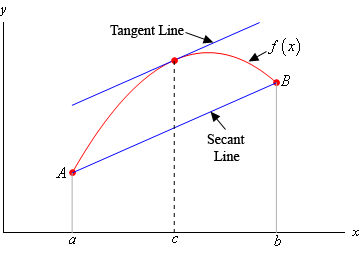
\includegraphics[scale=0.65]{img/cap4.png}
    \caption{\footnotesize Representación gráfica del teorema del valor medio para derivadas.}
    \label{fig:tvmd}
\end{figure}

Ahora, nuestra tarea es ver el teorema del valor medio para las integrales. Sin embargo, necesitamos un resultado previo para poder establecerlo:

\begin{teo}[Teorema de los valores intermedios]
    Sea $f: [a,b] \rightarrow \R$ continua. Si $f(a) \neq f(b)$, entonces para cada $\beta \in f([a,b])$ existe al menos un $c \in (a,b)$ tal que $f(c) = \beta$.
\end{teo}

\begin{figure}
    \centering
    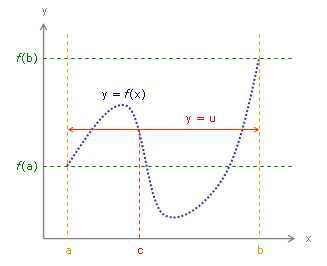
\includegraphics[scale=0.75]{img/cap5.png}
    \caption{\footnotesize Representación gráfica del teoremad de los valores intermedios}
    \label{fig:tvi}
\end{figure}

\marginnote{Estos dos teoremas se ven en los cursos anteriores de cálculo y en Análisis I.}

\begin{teo}[Teorema del valor medio (versión para integrales)]
    Sean $f,g: [a,b] \rightarrow \R$ continua con $f(x) > 0$ para todo $x \in [a,b]$, entonces existe $c \in (a,b)$ tal que
    
    \[
    \intab g(x)f(x)dx = g(c)\intab f(x)dx
    \]
\end{teo}

\begin{proof}
    Como $g$ es continua y cerrada en el intervalo $[a,b]$, es acotada y podemos tomar su máximo y mínimo. Entonces, sean
    
    \[
    M = \max_{x \in [a,b]} g(x) \qquad m = \min_{x \in [a,b]} g(x)
    \]
    
    Ahora, por la propiedad de monotonía de las integrales podemos establecer la siguiente cadena de desigualdades:
    
    \begin{gather*}
        m \leq g(x) \leq M \implies mf(x) \leq g(x)f(x) \leq Mf(x) \\
        \implies m\intab fdx \leq \intab fgdx \leq M\intab fdx
    \end{gather*}
    
    Como $f(x) > 0$, entonces por propiedad de positividad $\intab fdx > 0$, y la desigualdad anterior queda de la siguiente manera
    
    \begin{equation}\label{eq:cocint}
        m \leq \dfrac{\intab fgdx}{\intab fdx} \leq M
    \end{equation}
    
    Por otro lado, por el teorema de los valores intermedios, podemos garantizar la existencia de $x_0, x_1 \in [a,b]$ tales que
    
    \[
    g(x_0) = m \qquad g(x_1) = M
    \]
    
    \noindent de esta forma, como el cociente $\displaystyle \dfrac{\intab fgdx}{\intab fdx} \in g([a,b])$, existe $c \in [a,b]$ tal que
    
    \[
    \dfrac{\intab fgdx}{\intab fdx} = g(c) \implies \intab fgdx = g(c)\intab fdx
    \]
    
    \noindent y hemos llegado al resultado querido, y el teorema queda demostrado.
\end{proof}

\begin{cor}
    Si $g$ es continua en $[a,b]$ entonces existe un $c$ en $[a,b]$ tal que
    
    \[
    g(c) = \frac{1}{b-a} \intab g(x)dx
    \]
\end{cor}

\begin{proof}
    Basta tomar $f \equiv 1$, luego por el teorema del valor medio,
    
    \[
    \intab fgdx = g(c)\intab fdx \iff \intab gdx = (b-a)g(c) \iff g(c) = \frac{1}{b-a} \intab g(x)dx
    \]
\end{proof}

\begin{figure}
    \centering
    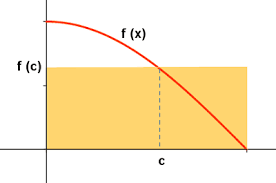
\includegraphics[scale=0.75]{img/cap6.png}
    \caption{\footnotesize Lo que sucede con el teorema del valor medio para las integrales es lo siguiente: Hay un $c \in [a,b]$ tal que el rectángulo de altura $g(c)$ tiene área igual al área bajo la curva de $g(x)$.} 
    \label{fig:my_label}
\end{figure}